\documentclass[12pt]{exam}

\usepackage{amssymb}
\usepackage{mathtools}
\usepackage{algorithm}
\usepackage{float}  % Figure placement
\usepackage{minted}  % Code highlighting
\usepackage{tikz}  % Flow chart
\usepackage{lipsum}
\usepackage{xspace}
\usepackage{hyperref}
\usepackage{MnSymbol}
\usepackage{pgffor}
\usepackage{mdframed}


\hypersetup{
    colorlinks = true,
    linkcolor = blue,
    urlcolor  = blue,
    citecolor = blue,
    anchorcolor = blue
}

\newcommand{\hwheaderfooter}[3]{
\pagestyle{headandfoot}
\firstpageheadrule
\firstpageheader{#1}{#2}{#3}
\runningheader{#1}{#2}{#3}
\runningheadrule
\firstpagefooter{}{\thepage}{}
\runningfooter{}{\thepage}{}
}

\newcommand{\latex}{\LaTeX\xspace}

\newcommand{\stars}[1]{%
    \foreach \n in {1,...,#1}{%
        $\filledstar$%
    }%
}

\hwheaderfooter{HW 4}{}{CSCI 406}


\begin{document}
\begin{center}
  \fbox{\fbox{\parbox{\textwidth - 0.2 in}{\centering

{Instructions: Please note that handwritten assignments \textbf{will not be graded}. Use the 
provided \latex template to complete your homework. Please do not alter the order or spacing of 
questions (keep each question on its own page). When you submit to Gradescope, you must mark 
which page(s) correspond to each question. \textbf{You may not receive credit for unmarked 
questions}. \\ When including graphical figures, we encourage the use of tools such as \href{https://dreampuf.github.io/GraphvizOnline/}{graphviz} or packages like \href{https://www.overleaf.com/learn/latex/TikZ_package}{tikz} for simple and complex figures. However, these may be handwritten only if they are neat and legible (as defined by the grader). }\\

}}}
\end{center}

\textbf{List any collaborators (besides TAs or professors) here:}

\begin{questions}
\question[10] [W5] For the following questions, select the true statement(s). \textbf{No explanation is necessary for these questions.}

\begin{parts}
    \part What is true about the residual graph in the Ford-Fulkerson algorithm?

    % Replace \square with \blacksquare for the option(s) you would like to select.
    $\bblacksquare$ The sum of residual capacities over all edges in the residual graph is equal to the sum of the capacities in the original graph. \\
    $\square$ The number of edges in the residual graph is at least equal to the number of directed edges in the flow network. \\
    $\square$ The capacity of any edge in residual graph does not exceed the capacity of the corresponding edge in the flow network, if it exists. \\
    $\square$ The capacity of an edge in the residual graph depends on the direction, quantity, and capacities of the pipes between the two vertices.

    % Replace \square with \blacksquare for the option(s) you would like to select.
    \part What must be true if there is a directed path in the residual graph from the source to the sink in the Ford-Fulkerson algorithm?

    $\square$ The flow is not maximized. \\
    $\square$ The path is an augmenting path. \\
    $\square$ There is a cut in the original flow graph whose capacity is equal to the flow in the network.
\end{parts}

\clearpage

\question[10] [W5] Flow. For the following questions, select whether the statement is true or false,
    and write a \textit{brief} explanation of your reasoning (no more than two sentences).
\begin{parts}
    % Replace \square with \blacksquare for the option(s) you would like to select.
    \part The maximum flow in a flow network is equal to the minimum cut of the network.\\
    $\square$ True $\square$ False

    \part In the residual graph of the maximum flow, there are no augmenting paths from the source to the sink. \\
    $\square$ True $\square$ False

    \part In a residual network, the capacity of an edge can be zero.\\
    $\square$ True $\square$ False

    \part If a single edge's capacity in a flow network is increased, the maximum flow value can only either stay the same or increase.\\
    $\square$ True $\square$ False

    
\end{parts}

\clearpage

\question[15] [W5] How can standard, unmodified max-flow algorithms (which only work with a single source and single sink node) be applied to a graph with multiple sources and sinks? Describe the necessary steps or considerations. (Expected answers are a few sentences long [a short paragraph].)


\clearpage

\question[40] [W5] 
After the Titanic collided with an iceberg, many people were able to evacuate.
However, not all were able to escape the wreckage.
You are given a grid of the following symbols:
\begin{itemize}
    \item \texttt{*} - Exactly one person on a piece of floating ice.
    % This person wants to escape from this piece of ice as soon as possible.
    After the person leaves, the piece of ice sinks (and no one else can use it).
    \item \texttt{W} - Water. People cannot move through the water because it is extremely cold.
    \item \texttt{i} - A small piece of floating ice. Exactly one person can move to a floating piece of ice and wants to escape from it as soon as possible. After the person leaves, the piece of ice sinks (and no one else can use it).
    \item \texttt{@} - Large Iceberg. At most one person can be on this iceberg at a time, but it will not sink after that person leaves.
    \item \texttt{\%} - Lifeboat. These are stationary boats that can hold at most 5 people.
\end{itemize}
People can move to the 4 cardinal adjacencies of their current square (N, S, E, W).
\textbf{Your goal is to get as many people as possible to the lifeboats, where they can stay until other ships arrive.}

Considering the following instance of this problem:
\vspace{0.8cm}
{
\large
\begin{center}
    \texttt{*\hspace{1.5 cm}W\hspace{1.5 cm}W\hspace{1.5 cm}\%} \\ \vspace{1 cm}
    \texttt{i\hspace{1.5 cm}i\hspace{1.5 cm}@\hspace{1.5 cm}@} \\ \vspace{1 cm}
    \texttt{W\hspace{1.5 cm}W\hspace{1.5 cm}i\hspace{1.5 cm}*} \\ \vspace{1 cm}
    \texttt{i\hspace{1.5 cm}W\hspace{1.5 cm}i\hspace{1.5 cm}*} \\ \vspace{1 cm}
\end{center}
}

\begin{parts}
    \part[5] For the above instance, what is the maximum number
        of people that can make it to a lifeboat.

    \textbf{Answer:} 

    \part[10] What graph algorithm would you use to solve this problem?
        Like the maze project, you may \textbf{not} modify the underlying algorithm
        at all (you must encode/model all of the information for the
        problem in the graph). \vspace{0.3cm} \\
        % Replace \square with \blacksquare for the option(s) you would like to select.
        $\square$ BFS \\
        $\square$ DFS \\
        $\square$ Ford Fulkerson or Edmonds-Karp \\
        $\square$ Dijkstra's \\
        $\square$ Prim's or Kruskal's \\
        $\square$ Floyd-Warshall

    \part[25] Draw the graph
        that you would use to solve the instance of the problem given on
        the last page.

\end{parts}



\clearpage
\question[15] [W6] Bipartite Matching. For the following questions, select whether the statement is true or false,
    and write a \textit{brief} explanation of your reasoning (between one and three sentences).

    \textbf{For all of these questions $G = (V, E)$ is a bipartite graph and $X$ and $Y$ are
    the subsets $G$ such that all edges have one endpoint in $X$ and one in $Y$.
    The graph $H$ is the flow network used in the reduction to max flow as described in class.}

    \begin{parts}
    % Replace \square with \blacksquare for the option(s) you would like to select.
    \part Any valid solution to the maximum bipartite matching problem for $G$ contains exactly $\min(|X|, |Y|)$ edges.\\
        $\square$ True 
        $\square$ False

    \part There are $|X| + |Y| + |E|$ edges in $H$.\\
        $\square$ True 
        $\square$ False

    \part After computing the max flow of $H$, all edges in $H$ with flow of 1 constitute the solution to
        the maximum bipartite matching problem for $G$.\\
        $\square$ True 
        $\square$ False

    \part If an augmenting path exists in the residual graph of $H$, then the current matching in $G$ is not maximum.\\
        $\square$ True 
        $\square$ False
        
    \part The complexity of solving the maximum bipartite matching problem using the max flow reduction
        discussed in class is $\mathcal{O}(|V| \times |E|)$.\\
        $\square$ True 
        $\square$ False 
        \hspace{0.5in} \textbf{No explanation necessary for this problem}
    
    \end{parts}

    \clearpage



\question[10] [AlgoBOWL] The following questions are about the AlgoBOWL project. For the following questions, select whether the statement is true or false. \textbf{No explanation is necessary for these problems.}

\begin{parts}
    \part My team should expect to compute an optimal solution for every input with our algorithm.
    
        % Replace \square with \blacksquare for the option you would like to select.
        $\square$ True 
        $\square$ False

    \part For an output from another team to be valid, it must match my team's output.
    
        % Replace \square with \blacksquare for the option you would like to select.
        $\square$ True 
        $\square$ False

    \part If there are $k$ groups in your AlgoBOWL section (including your group), your group will 
    need to:
    
    
        % Replace \square with \blacksquare for the option you would like to select.
        $\square$ Supply one input, compute $k$ outputs and perform $k$ verifications (not including open verification).\\
        $\square$ Supply one input, compute $k-1$ outputs and perform $k-1$ verifications (not including open verification).\\
        $\square$ Supply one input, compute $k$ outputs and perform $k^2$ verifications (not including open verification).\\
        $\square$ Supply one input, compute one output and perform one verification (not including open verification).

        \part Placing NO tents is a valid solution to the AlgoBOWL problem.
    
        % Replace \square with \blacksquare for the option you would like to select.
        $\square$ True 
        $\square$ False

    \part For the solution below, the first line of the output should $8$.
        % Replace \square with \blacksquare for the option you would like to select.
        
        $\square$ True 
        $\square$ False 

        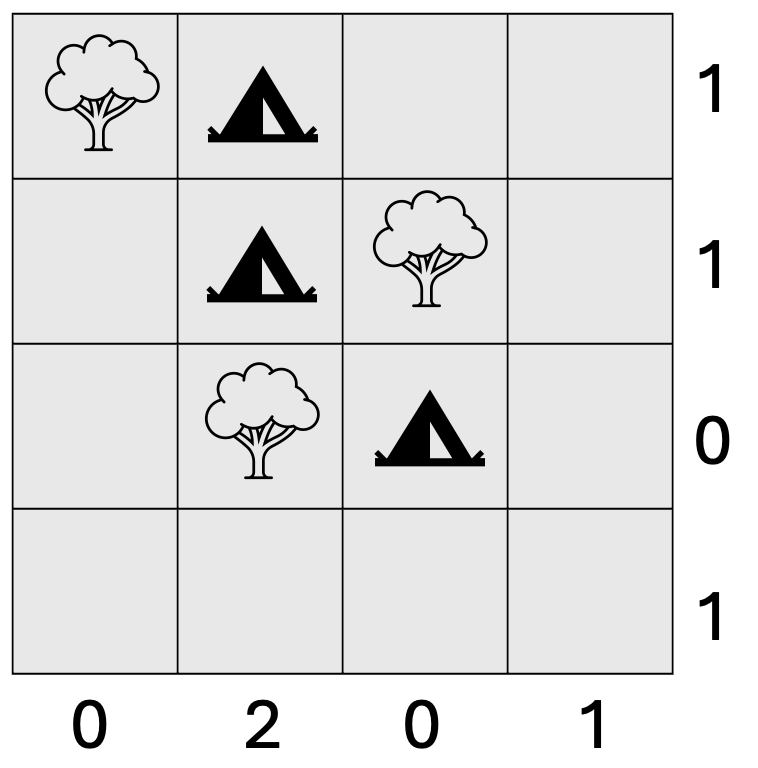
\includegraphics[width=0.25\textwidth]{algobowl_tandt.png}


\end{parts}

% close the document
\end{questions}
\end{document}
